\documentclass{article}
\setlength{\parindent}{0in}
\usepackage[
bottom = 2.50cm,
left   = 2.50cm,
right  = 2.50cm]{geometry}
\newcommand{\code}{\texttt}

\usepackage{graphicx}% Include Fig. files
\usepackage{dcolumn}% Align table columns on decimal point
\usepackage{bm}% bold math
\usepackage{caption}
\usepackage[labelformat=simple]{subcaption}
\usepackage{float}
\usepackage{amsmath}
\usepackage{amssymb}
\usepackage[export]{adjustbox}
\usepackage[dvipsnames]{xcolor}
\usepackage{authblk}
\usepackage{url}

\begin{document}

\title{ESC407 Lab 1}

\author{Maggie Wang}

\date{October 2, 2023}
\maketitle

\begin{enumerate}
\item Diffraction
\begin{enumerate}
    \item 
    
    The procedure to numerically compute the Bessel function $J_m(x)$ using Simpson's rule is outlined below. Fig. \ref{fig:1a} shows the results for Bessel functions $J_0$, $J_1$, and $J_2$ as a function of $x$ from $x=0$ to $x=2$.
    
    \begin{figure}[H]
        \centering
        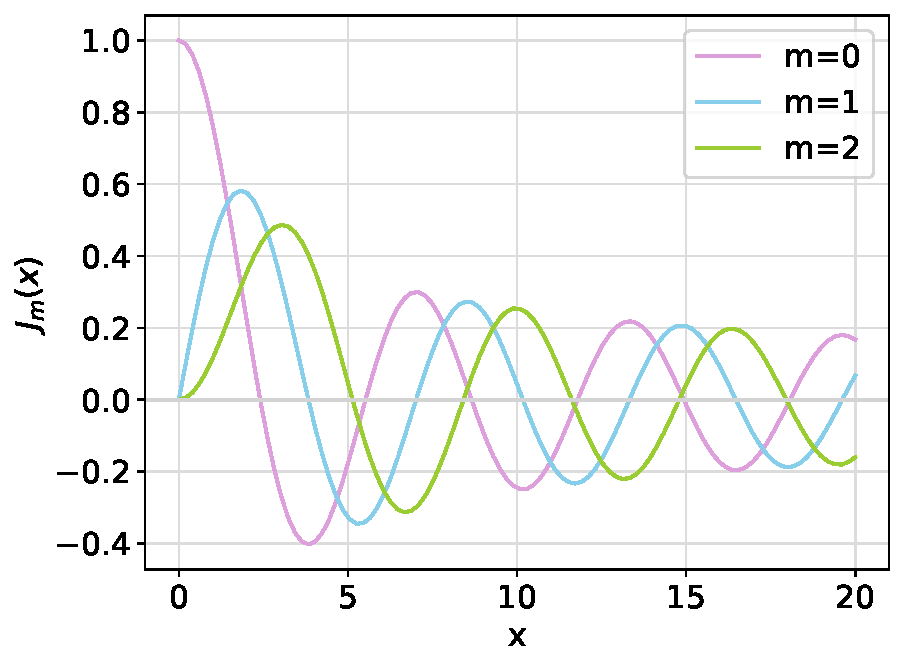
\includegraphics[width=0.6\linewidth]{1a.pdf}
        \caption{\label{fig:1a} Bessel functions $J_m(x)$ computed using Simpson's rule}
    \end{figure} 

    \textbf{Pseudocode}\\
    Simpson's rule 
    \begin{itemize}
        \item Define function \code{simpson(N, a, b, f)}, which computes Simpson's rule on some function \code{f} over \code{[a, b]} with \code{N} integration points
        \begin{itemize}
            \item Compute step size \code{h = (b-a)/N }
            \item Initialize \code{sum\_f} with value \code{f(a) + f(b)}
            \item For each integer \code{k} from 1 to \code{N}:
            \begin{itemize}
                \item If \code{k} is even, add \code{2f(a+kh)} to \code{sum\_f}
                \item If \code{k} is odd, add \code{4f(a+kh)} to \code{sum\_f}
            \end{itemize}
            \item Return \code{h*sum\_f/3}
        \end{itemize}
    \end{itemize}
    
    Bessel function
    \begin{itemize}
        \item Define function \code{J\_integrand(theta, m, x)}
        \begin{itemize}
            \item Return \code{cos(m theta - x sin(theta))}
        \end{itemize}
        \item Define function \code{J(m, x)}
        \begin{itemize}
            \item Call \code{simpson} with arguments \code{N}=1000, \code{a}=0, \code{b}=$\pi$, and \code{f=J\_integrand(theta, m=m, x=x)}
        \end{itemize}
    \end{itemize}

    Plotting 
    \begin{itemize}
        \item Initialize and set the number of plotted points \code{nvals=100}
        \item For each value of \code{m}:
        \begin{itemize}
            \item Initialize \code{x\_arr} with \code{nvals} equally spaced points between 0 and 20
            \item Compute \code{y\_arr} as \code{J(m, x)} for each \code{x} in \code{x\_arr}
            \item Plot \code{y\_arr} vs \code{x\_arr}
        \end{itemize}
    \end{itemize}

    \item The calculation using Simpson's rule closely matches results using \code{scipy.special.jv}, as seen in Fig. \ref{fig:1b}. The pseudocode to generate Fig. \ref{fig:1b} is outlined below.
    
    \begin{figure}[H]
        \centering
        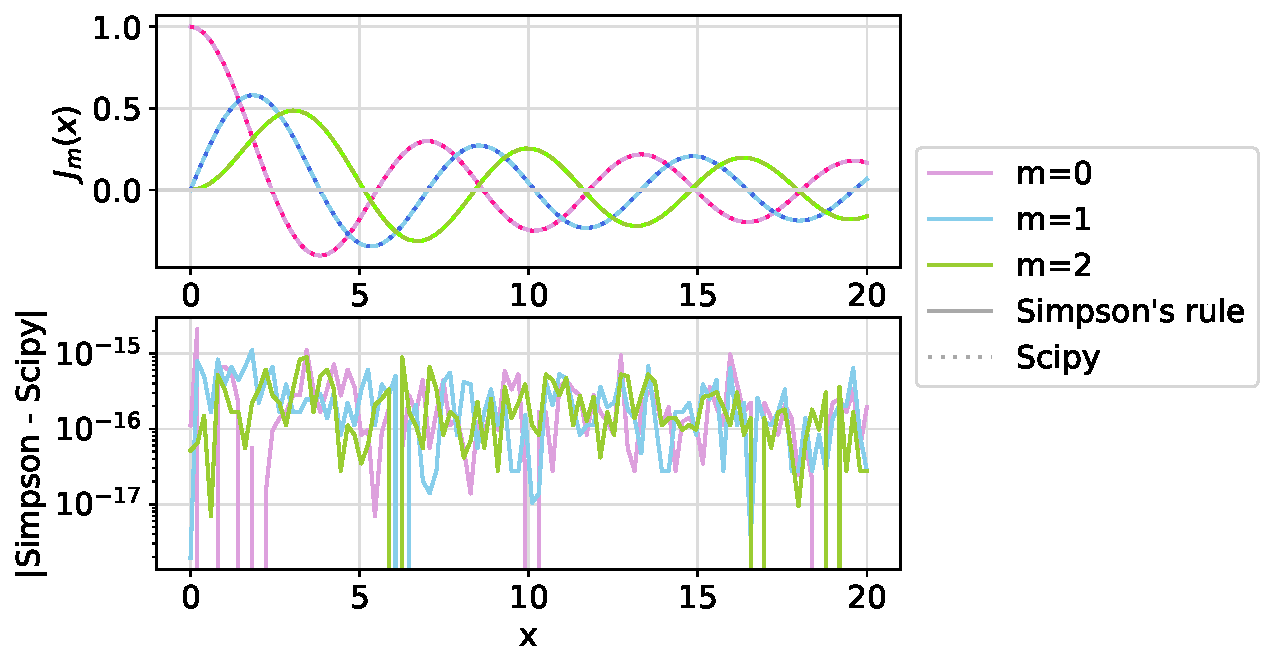
\includegraphics[width=0.8\linewidth]{1b.pdf}
        \caption{\label{fig:1b} Bessel functions $J_m(x)$ computed using Simpson's rule and \code{scipy.special.jv}}
    \end{figure} 

    \textbf{Pseudocode}
    \begin{itemize}
        \item Initialize and set \code{nvals=100}
        \item For each value of \code{m} of interest:
        \begin{itemize}
            \item Initialize \code{x\_arr} with \code{nvals} equally spaced points between 0 and 20
            \item Computearrays \code{J\_simpson} as \code{J(m, x)} and Compute \code{J\_scipy} using Scipy functions for each \code{x} in \code{x\_arr}
            \item Plot \code{J\_simpson} and \code{J\_scipy} vs \code{x\_arr}
        \end{itemize}
    \end{itemize}

    \item Figure \ref{fig:1c} shows a plot of the intensity of the diffraction pattern from a point light source with $\lambda=500$ nm in the focal plane of a telescope, with Bessel functions computed using Simpson's rule. The pseudocode for the program which generates the plot is outlined below.
    
    \begin{figure}[H]
        \centering
        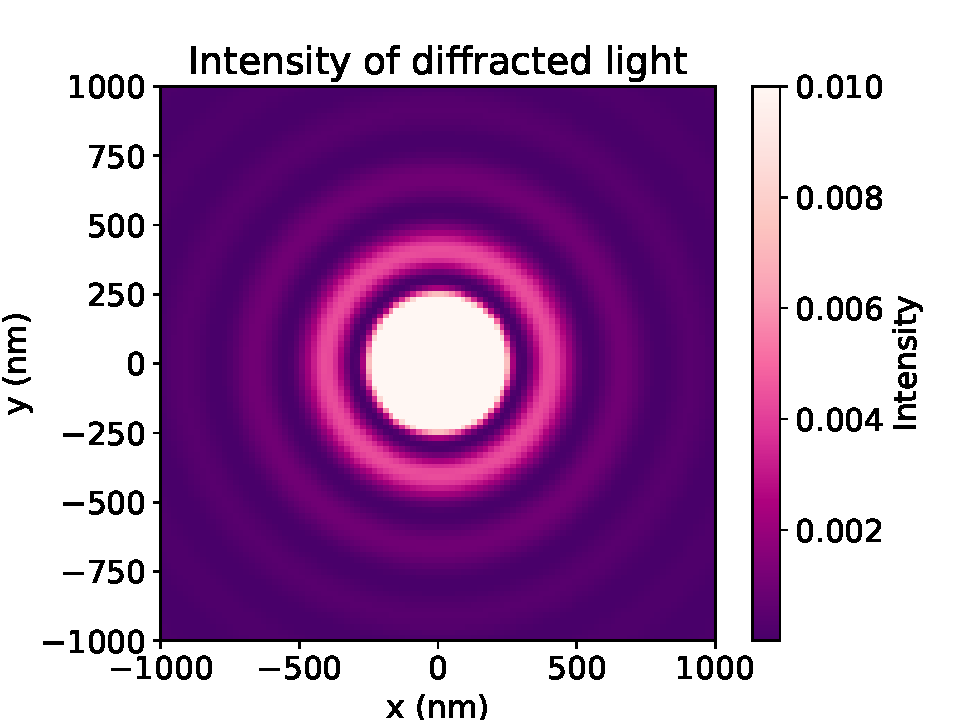
\includegraphics[width=0.6\linewidth]{1c.pdf}
        \caption{\label{fig:1c} Intensity of diffracted light from 500 nm point source over a radius of 1 um}
    \end{figure} 

    \textbf{Pseudocode}
    \begin{itemize}
        \item Define function \code{I(r, wavelength)}
        \begin{itemize}
            \item Return $\frac{J(2 \pi r /\text{wavelength})}{(2 \pi r /\text{wavelength})}^2$
        \end{itemize}
        \item Initialize and set \code{num\_grid\_points=100}, \code{wavelength=500} nm, radius \code{R=1000} nm
        \item Initialize arrays \code{x\_arr} and \code{y\_arr} with \code{nvals} evenly spaced values from -\code{R} to \code{R}
        \item Compute a 2D array \code{r\_mtx} with entries $x^2+y^2$, for \code{x} in \code{x\_arr} and \code{y} in \code{y\_arr}, representing the radial distance from the beam centre
        \item Compute a 2D array \code{intensity\_mtx} with entries \code{I(r, wavelength)} for each \code{r} in \code{r\_matrix}
    \end{itemize}

    \end{enumerate}

\item Trapezoidal and Simpson’s rules for integration
\begin{enumerate}
    \item Table \ref{tab:2a} summarizes the value of the Dawson function at $x=4$ computed using Simpson's and trapezoidal rules with 8 integration slices, and \code{scipy.special.dawsn}.

    \begin{table}[H]
    \centering
    \begin{tabular}{c|c|c}
        Simpson's rule & Trapezoidal rule & Scipy \\\hline 
        0.1826909645971217 & 0.26224782053479523 & 0.1293480012360051
    \end{tabular}
    \captionsetup{width=0.65\textwidth}
    \caption{Value of Dawson function at $x=4$ computed using Simpson's and trapezoidal rules with 8 slices, and with \code{scipy.special.dawsn}}
    \label{tab:2a}
    \end{table}

    \item Table \ref{tab:2b} summarizes the number of slices needed to approximate the Dawson function at x=4 with an error $\mathcal{O}(10^{-9})$, and the corresponding run time. $scipy.special.dawsn$ was used as the reference value, and the runtime of each method was averaged over 50 calls. 
    
    \begin{table}[H]
        \centering
        \begin{tabular}{c|c|c|c|c}
            \centering
            & N & runtime (ms) & value & error \\\hline 
            Simpson's rule & 1024 & $0.845$ & 0.12934800196026494 & $7.242598465406758\times 10^{-10}$\\\hline
            Trapezoidal rule & 65536 & $48$ & 12934800371953178 & $2.483526689855964\times 10^{-9}$ \\ 
        \end{tabular}
    \captionsetup{width=0.9\textwidth}
    \caption{Number of integration slices (N), corresponding runtime, output, and error required to approximate $D(4)$ to $\mathcal{O}(10^{-9})$, with $scipy.special.dawsn$ used as a reference value.}
    \label{tab:2b}
    \end{table}

    \item Using $N_2$ = 64 and $N_1$ = 32, the error estimate of D(4) using Simpson's rule is 
        \begin{align*}
            \epsilon_2& = \frac{1}{15}(I_2-I_1) \\
            &= 0.00020578842293380212,
        \end{align*}
    and for trapezoidal rule, 
        \begin{align*}
            \epsilon_2 &= \frac{1}{3}(I_2-I_1) \\
            &= 0.0005093137305911358
        \end{align*}
\end{enumerate}

\item Exploring roundoff error
\begin{enumerate}
    \item Fig. \ref{fig:3a} shows $p(u)=(1-x)^8$ and $q(u)$, the Taylor expansion of $p(u)$ up to degree 8. The plot of $q(u)$ appears noisier because there are more terms involved which are each affected by roundoff error.
    \begin{figure}[h]
        \centering
        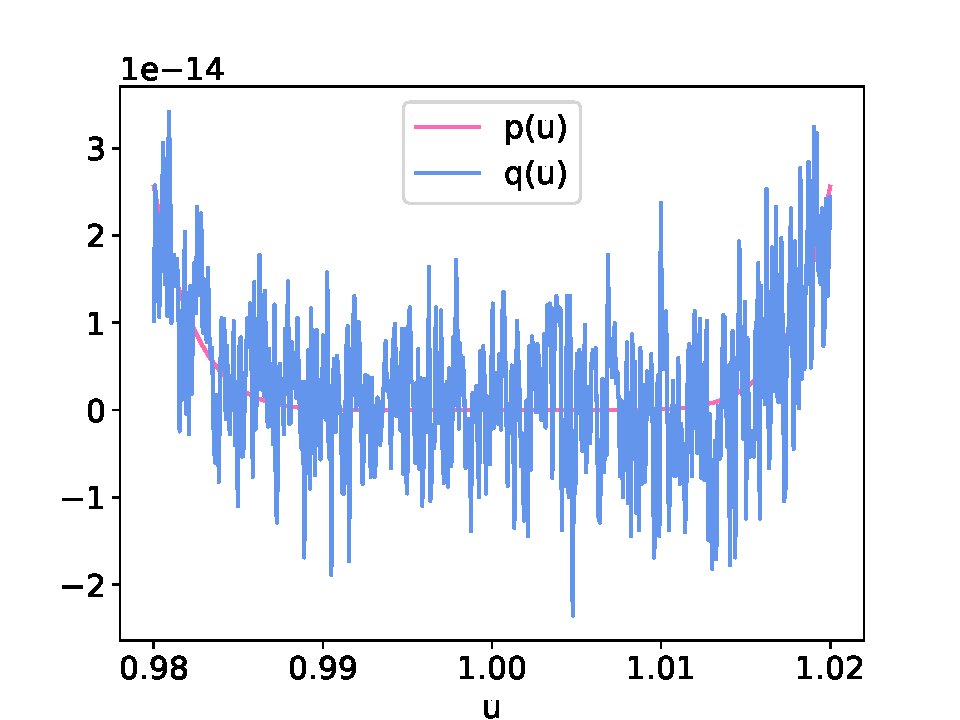
\includegraphics[width=0.7\textwidth]{3a.pdf}
        \caption{$p(u) = (1-x)^8$ and its Taylor expansion to degree 8, $q(u)$, around u = 1}
        \label{fig:3a}
    \end{figure} 

    \item Fig. \ref{fig:3b} a) plots $|p(u)-q(u)|$ around u = 1. Fig. \ref{fig:3b} b) shows the histogram associated with Fig. \ref{fig:3b} a), which has a standard deviation of $8\times10^{-15}$. This standard deviation should be the same order of magnitude as an estimate obtained using equation 1, since they are both measures of roundoff error when summing over multiple terms.

    \begin{figure}[h]
        \centering 
        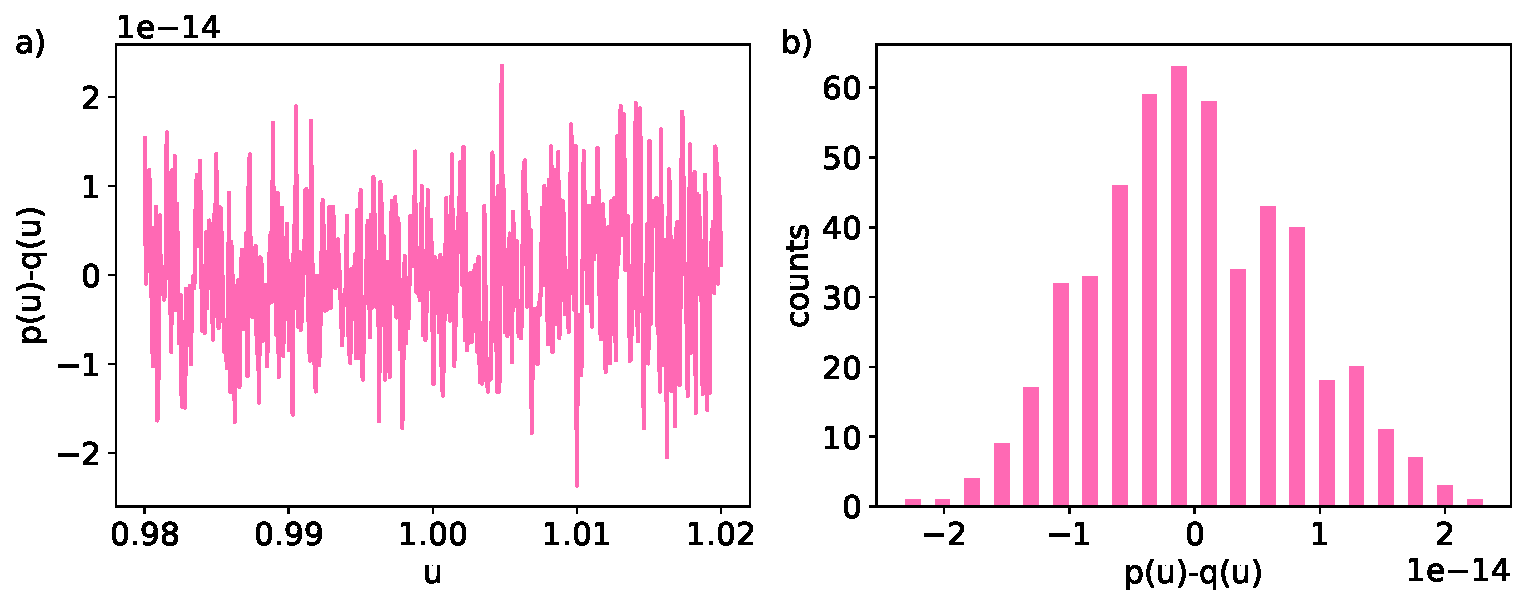
\includegraphics[width=\textwidth]{3b.pdf}
        \caption{a) $|p(u)-q(u)|$ around u = 1 and b) the corresponding histogram}
        \label{fig:3b}
    \end{figure}

    The estimate of the error obtained using equation 1 for $p(1)-q(1)$ is the same order of magnitude as the standard deviation above.
    \begin{align*}
        \sigma &= C\sqrt{N}\sqrt{\bar{x^2}}\\
        &= 10^{-16}\sqrt{10}\sqrt{1287}\\
        &= 1.1 \times 10^{-14}
    \end{align*}
    The operation $p(u)-q(u)$ is a sum over $p(u)$ and each term in $q(u)$, for $u=1$. Since there are 10 terms in total, $N=10$. $\bar{x^2}$ is calculated as 
    \begin{align*}
        \bar{x^2} &= \frac{(1-1)^{8\cdot 2} + 1^2 + 8^2 + 28^2 + 56^2 + 70^2 + 56^2 +28^2 + 8^2+ 1^2}{10}\\
        &= 1287
    \end{align*}
    
    \item Equation 2 estimates the fractional error as
    \begin{align*}
        \frac{\sigma}{\sum_i x_i} &= \frac{C}{\sqrt{N}}\frac{\sqrt{\bar{x^2}}}{\bar{x}}
    \end{align*}
    In the calculation of $p(u)-q(u)$, the $x_i$'s alternates sign and as a result, $\bar{x}$ is much smaller than $\sqrt{\bar{x^2}}$ and the fractional error becomes quite large. 
    Using $N=10$ and the same method to calculate $\bar{x^2}$ as above, for $u=0.985$,
    \begin{align*}
        \sqrt{bar{x^2}} &= 33.778\\
        \bar{x} &= 2.232\times 10^{-15}\\
        \frac{\sigma}{\sum_i x_i} &= 0.478
    \end{align*}
    For $u=0.99$,
    \begin{align*}
        \sqrt{bar{x^2}} &\approx 34.465\\
        |\bar{x}\ &= 1.898 \times 10^{-16}\\
        |\frac{\sigma}{\sum_i x_i}| &= 5.741
    \end{align*}

    Between $u=0.985$ and $u=0.99$, the estimated fractional error approaches 1.00

    Fig. \ref{fig:3c} shows that the fractional error $|p(u)-q(u)|/p(u)$ approaches 1.00 when $u$ is between 0.978 and 0.985

    \begin{figure}[h]
        \centering
        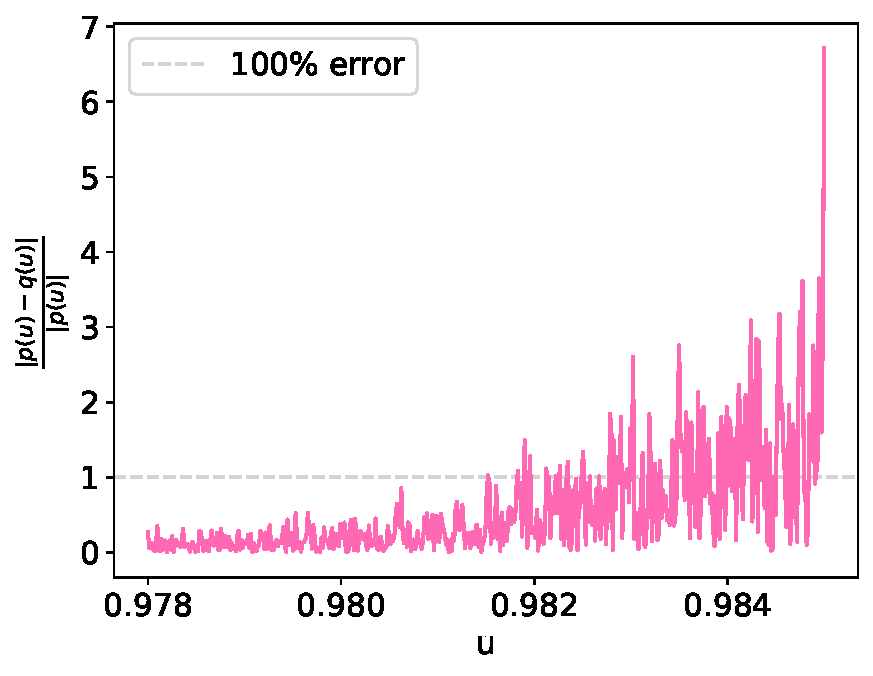
\includegraphics[width=0.6\textwidth]{3c.pdf}
        \caption{Fractional error $|p(u)-q(u)|/p(u)$ for $u$ between 0.978 and 0.985}
        \label{fig:3c}
    \end{figure}

    \item Plotting $u^8/(u^4u^4)-1$ shows the error is on the order of $10^{-16}$, which is the same as what equation (4.5), $\sigma = \sqrt{2}C x = 1.41\times10^{-16}$, predicts for $C=10^{-16}$ and $x=1$
    \begin{figure}[h]
        \centering 
        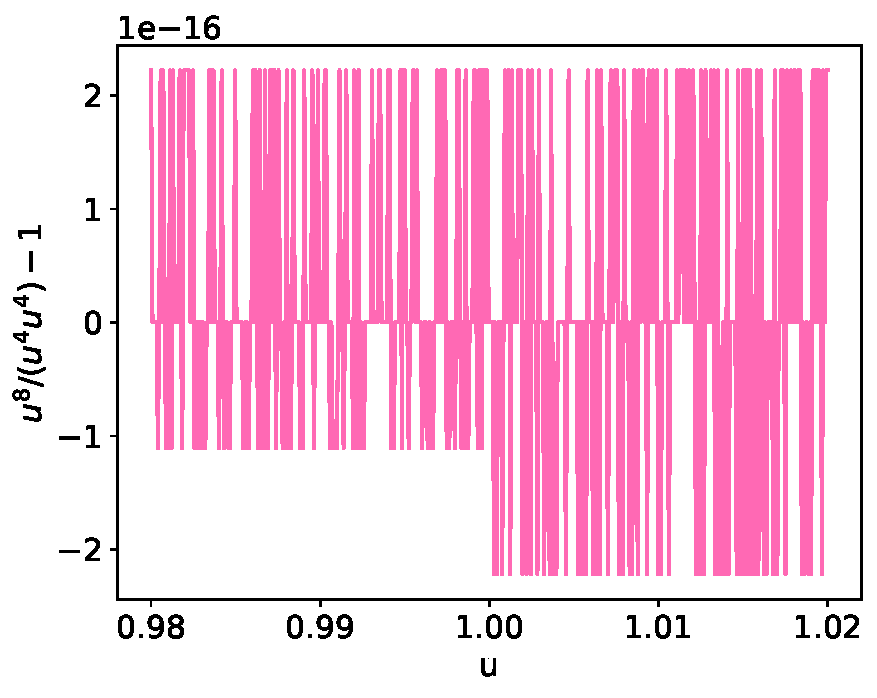
\includegraphics[width=0.6\textwidth]{3d.pdf}
        \caption{$u^8/(u^4u^4) - 1$ around u=1}
        \label{fig:3d}
    \end{figure}

\end{enumerate}

\end{enumerate}


\end{document}